\documentclass{standalone}

\usepackage{tikz}
\usetikzlibrary{arrows,positioning,shapes,automata,backgrounds,petri,fit,matrix,decorations.pathreplacing,calc}

\usepackage{minted}
\newminted[cppcode]{cpp}{autogobble,breaklines}

\usepackage{xcolor}
\colorlet{mygreen}{green!60!black}

\begin{document}
    \begin{minipage}[c]{0.22\textwidth}
      \begin{cppcode}
        int x = 0;
        int y = 0;

        void T1() {
          y = 1;
          int a = x;
        }
        void T2() {
          x = 1;
          int b = y;
        }
      \end{cppcode}
    \end{minipage}
    %
    \hfill
    %
    \begin{minipage}[c]{0.77\textwidth}
    \begin{center}
    \noindent
    Is $a = 0 \land b = 0$ reachable?\\[2.5ex]
    \medskip
    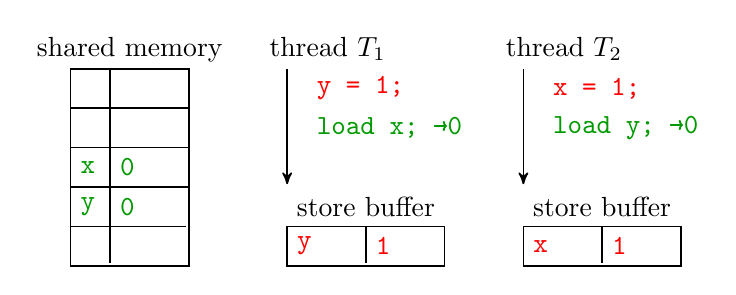
\begin{tikzpicture}[ ->, >=stealth', shorten >=1pt, auto, node distance=3cm
                       , semithick
                       , scale=0.5
                       ]

      \draw [-] (-10,0) rectangle (-7,-5);
      \draw [-] (-10,-1) -- (-7,-1)
                (-10,-2) -- (-7,-2)
                (-10,-3) -- (-7,-3)
                (-10,-4) -- (-7,-4);
      \draw [-] (-9,0) -- (-9,-5);
      \node () [] at (-8.5,0.5) {shared memory};
      \node () [anchor=west] at (-10,-2.5)  {\texttt{\color{mygreen}x}};
      \node () [anchor=west] at (-9,-2.5) {\texttt{\color{mygreen}0}};

      \node () [anchor=west] at (-10,-3.5)  {\texttt{\color{mygreen}y}};
      \node () [anchor=west] at (-9,-3.5)  {\texttt{\color{mygreen}0}};

      \node () [anchor=center] at (-2.5,-3.5) {store buffer};
      \draw [-] (-4.5,-4) rectangle (-0.5,-5);
      \draw [-] (-2.5,-4) -- (-2.5,-5);

      \node () [anchor=center] at (3.5,-3.5) {store buffer};
      \draw [-] (1.5,-4) rectangle (5.5,-5);
      \draw [-] (3.5,-4) -- (3.5,-5);

      \node () [anchor=west] at (-4.5,-4.5)  {\texttt{\color{red}y}};
      \node () [anchor=west] at (-2.5,-4.5)  {\texttt{\color{red}1}};

      \node () [anchor=west] at (1.5,-4.5)  {\texttt{\color{red}x}};
      \node () [anchor=west] at (3.5,-4.5)  {\texttt{\color{red}1}};

      \node () [anchor = west, xshift = -1em] at (-4.5, 0.5) {thread $T_1$};
      \draw [->] (-4.5,0) -- (-4.5,-3);
      \node () [anchor=west] at (-4, -0.5) {\texttt{\color{red}y = 1;}};
      \node () [anchor=west] at (-4, -1.5) {\texttt{\color{mygreen}load x; \textrightarrow 0}};

      \node () [anchor = west, xshift = -1em] at (1.5, 0.5) {thread $T_2$};
      \draw [->] (1.5,0) -- (1.5,-3);
      \node () [anchor=west] at (2, -0.5) {\texttt{\color{red}x = 1;}};
      \node () [anchor=west] at (2, -1.5) {\texttt{\color{mygreen}load y; \textrightarrow 0}};

  \end{tikzpicture}
  \end{center}
  \end{minipage}
\end{document}
